\documentclass[aspectratio=169, 10pt]{beamer}
\usetheme{Madrid}
\usecolortheme{default}

\usepackage[utf8]{inputenc}
\usepackage[T1]{fontenc}
\usepackage{lmodern}
\usepackage[english]{babel}
\usepackage{amsmath,amssymb,amsfonts}
\usepackage{booktabs}
\usepackage{colortbl}
\usepackage{xcolor}
\usepackage{tikz}
\usetikzlibrary{arrows.meta,positioning,shapes,calc}
\usepackage{pgfplots}
\pgfplotsset{compat=1.18}

\setbeamercovered{transparent}
\setbeamertemplate{navigation symbols}{}


\definecolor{geblue}{RGB}{31, 119, 180}
\definecolor{gebluemid}{RGB}{31, 119, 180}
\definecolor{cghred}{RGB}{214, 39, 40}
\definecolor{lightgeblue}{RGB}{165, 200, 224}
\definecolor{barlightblue}{RGB}{121, 173, 210}
\definecolor{dipgorange}{RGB}{255, 127, 14}
\definecolor{midlgreen}{RGB}{44, 160, 44}
\definecolor{midlbrown}{RGB}{147, 39, 39}
\definecolor{boxblue}{RGB}{221, 234, 243}
\definecolor{boxred}{RGB}{248, 222, 222}
\definecolor{boxgreen}{RGB}{223, 240, 223}
\definecolor{boxlavender}{RGB}{235, 237, 244}
\definecolor{cellgreen}{RGB}{171, 217, 171}
\definecolor{cellred}{RGB}{245, 201, 201}
\definecolor{celllightred}{RGB}{251, 233, 233}

\title[Pediatric Brain Tumor Localization]{Classification of Pediatric Brain Tumor Localization}
\subtitle{Multi-Omic Integration (Gene Expression + CGH) in the \texorpdfstring{$p \gg n$}{p >> n} Regime}
\author[]{R. Barata\texorpdfstring{\quad}{ }A. De Rouck\texorpdfstring{\quad}{ }M. Hoizey-Cangioloni\texorpdfstring{\quad}{ }P. Lubaszewski Lima\texorpdfstring{\quad}{ }M. Seyedi}
\institute[CentraleSupélec]{CentraleSupélec \\ \small Advisor: Arthur Tenenhaus}
\date[June 2026]{June 2026}

\pdfstringdefDisableCommands{%
  \def\quad{ }%
}

\AtBeginSection[]{
  \begin{frame}{Outline}
    \tableofcontents[currentsection]
  \end{frame}
}

\begin{document}

% Slide 1
\begin{frame}[plain]
  \titlepage
\end{frame}

% Slide 2
\begin{frame}{Presentation Outline}
  \tableofcontents
\end{frame}

% Slide 3: Section 1
\section{Introduction and Problem Formulation}

% Slide 4
\begin{frame}{Clinical Context and Problem Formulation}
  \begin{block}{The Problem}
    Predict the \textbf{anatomical localization} of a pediatric glioma strictly from the tumor's \textbf{molecular signature}.
    Localization strongly dictates surgical resectability, radiotherapy protocols, and overall patient prognosis.
  \end{block}

  \bigskip
  Three anatomical localizations define three target classes:
  \begin{itemize}
    \item \textbf{cort}: cortical / hemispheric tumors;
    \item \textbf{dipg}: diffuse intrinsic pontine glioma, located in the pons (inoperable, highly unfavorable prognosis);
    \item \textbf{midl}: midline tumors outside the pons (\textbf{rare class}).
  \end{itemize}
\end{frame}

% Slide 5
\begin{frame}{The Dataset}
  \begin{columns}[T]
    \begin{column}{0.48\textwidth}
      \textbf{Two molecular blocks:}\\
      \begin{itemize}
        \item \textcolor{geblue}{\textbf{GE}}: gene expression: \textbf{15,702} variables\\
              (primary discriminant signal);
        \item \textcolor{cghred}{\textbf{CGH}}: chromosomal gains / losses:\\
              \textbf{1,229} variables (weak signal in isolation).
      \end{itemize}

      \medskip
      \textbf{Sample size:} $n = 53$ patients: \textbf{39} in training and \textbf{14} in test.

      \medskip
      \begin{center}
        \small
        \begin{tabular}{lccc}
          \toprule
                         & \textbf{cort} & \textbf{dipg} & \textbf{midl}         \\
          \midrule
          \textbf{Train} & 15            & 16            & \textcolor{geblue}{8} \\
          \textbf{Test}  & 5             & 6             & \textcolor{geblue}{3} \\
          \bottomrule
        \end{tabular}
      \end{center}
    \end{column}

    \begin{column}{0.50\textwidth}
      \centering
      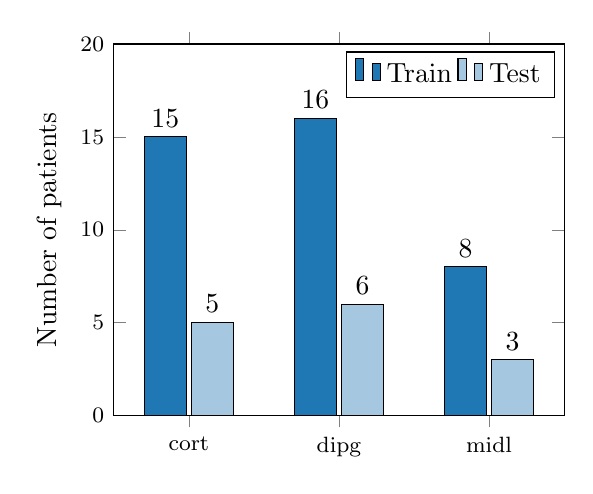
\begin{tikzpicture}
        \begin{axis}[
            ybar,
            width=7.3cm,
            height=6.3cm,
            bar width=15pt,
            ymin=0, ymax=20,
            ytick={0, 5, 10, 15, 20},
            ylabel={Number of patients},
            symbolic x coords={cort,dipg,midl},
            xtick=data,
            nodes near coords,
            nodes near coords style={/pgf/number format/fixed, /pgf/number format/precision=2},
            legend style={legend columns=2},
            enlarge x limits=0.25,
            tick label style={font=\footnotesize}
          ]
          \addplot[fill=geblue] coordinates {(cort, 15) (dipg, 16) (midl, 8)};
          \addplot[fill=lightgeblue] coordinates {(cort, 5) (dipg, 6) (midl, 3)};
          \legend{Train, Test}
        \end{axis}
      \end{tikzpicture}
      \vskip 2pt
        {\footnotesize Class distribution: midl is substantially under-represented.}
    \end{column}
  \end{columns}
\end{frame}

% Slide 6
\begin{frame}{The Statistical Challenge: Three Bottlenecks}
  \begin{columns}[T]
    \begin{column}{0.58\textwidth}
      \begin{enumerate}
        \item \textbf{Extreme $p \gg n$ regime}: $p = 16{,}931$ variables for $n = 39$ patients, yielding $\frac{p}{n} \simeq 434$. The Gram matrix $X^\top X$ has rank $\le n - 1 = 38$, hence is \emph{massively singular}: any unregularized estimator is non-identifiable.
        \item \textbf{Two heterogeneous and imbalanced blocks}: GE accounts for $92.7\%$ of variables; multi-block fusion must avoid marginalizing CGH.
        \item \textbf{Rare class midl}: 8 patients in train, 3 in test. Each error shifts its recall in steps of $1/3 \simeq 0.33$.
      \end{enumerate}
    \end{column}

    \begin{column}{0.40\textwidth}
      \begin{block}{Methodological Responses}
        \begin{itemize}
          \item $\ell_1 / \ell_2$ regularization + sparse feature selection;
          \item Block scaling + supervised latent projection (SGCCA);
          \item Likelihood weighting + \textbf{balanced accuracy}.
        \end{itemize}
      \end{block}
    \end{column}
  \end{columns}

  \vfill
  \begin{center}
    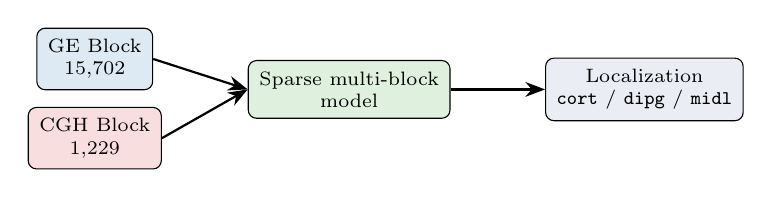
\begin{tikzpicture}[
      box/.style={rectangle, rounded corners=3pt, draw=black, align=center, font=\scriptsize, inner sep=4pt},
      arr/.style={-{Stealth[length=2.5mm]}, thick}
      ]
      \node[box, fill=boxblue] (ge) {GE Block \\ 15,702};
      \node[box, fill=boxgreen, right=1.2cm of ge, yshift=-11pt] (model) {Sparse multi-block \\ model};
      \node[box, fill=boxlavender, right=1.2cm of model] (loc) {Localization \\ \texttt{cort} / \texttt{dipg} / \texttt{midl}};
      \node[box, fill=boxred, below=6pt of ge] (cgh) {CGH Block \\ 1,229};

      \draw[arr] (ge.east) -- (model.west);
      \draw[arr] (cgh.east) -- (model.west);
      \draw[arr] (model.east) -- (loc.west);
    \end{tikzpicture}
  \end{center}
\end{frame}

% Slide 7: Section 2
\section{Exploratory Data Analysis (EDA)}

% Slide 8
\begin{frame}{GE Block Domination and Class Weighting}
  \vspace{14pt}
  \begin{columns}[c]
    \begin{column}{0.48\textwidth}
      \centering
      \hspace{5.5pt}%
      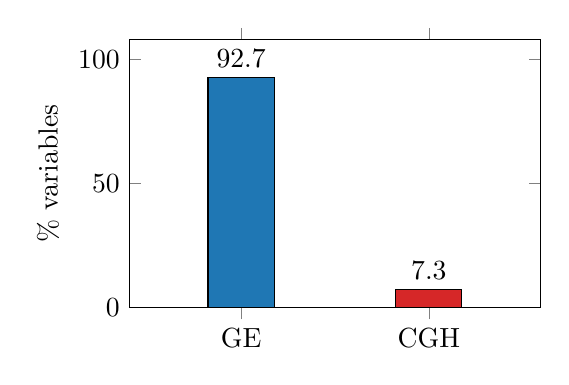
\begin{tikzpicture}
        \begin{axis}[
            ybar,
            width=5.22cm,
            height=3.40cm,
            scale only axis,
            bar width=23.9pt,
            ymin=0, ymax=108,
            ytick={0, 50, 100},
            ylabel={\% variables},
            symbolic x coords={GE,CGH},
            xtick={GE,CGH},
            nodes near coords,
            nodes near coords style={/pgf/number format/fixed, /pgf/number format/precision=1},
            enlarge x limits={abs=40.34pt},
          ]
          \addplot[fill=geblue, bar shift=0pt] coordinates {(GE, 92.7)};
          \addplot[fill=cghred, bar shift=0pt] coordinates {(CGH, 7.3)};
        \end{axis}
      \end{tikzpicture}
      \vskip 2pt
        {\footnotesize Inertia $\propto$ number of variables: raw concatenation is $> 90\%$ dominated by GE.}
    \end{column}

    \begin{column}{0.50\textwidth}
      \centering
      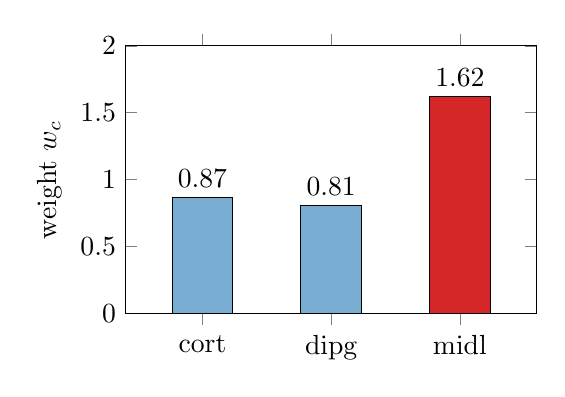
\begin{tikzpicture}
        \begin{axis}[
            ybar,
            width=5.22cm,
            height=3.40cm,
            scale only axis,
            bar width=21.9pt,
            ymin=0, ymax=2,
            ytick={0, 0.5, 1, 1.5, 2},
            ylabel={weight $w_c$},
            symbolic x coords={cort,dipg,midl},
            xtick={cort,dipg,midl},
            nodes near coords,
            nodes near coords style={/pgf/number format/fixed, /pgf/number format/precision=2},
            enlarge x limits={abs=27.74pt},
          ]
          \addplot[fill=barlightblue, bar shift=0pt] coordinates {(cort, 0.87) (dipg, 0.81)};
          \addplot[fill=cghred, bar shift=0pt] coordinates {(midl, 1.62)};
        \end{axis}
      \end{tikzpicture}
      \vskip 2pt
        {\footnotesize Inverse prevalence weights $w_c = n/(K\,n_c)$: a midl patient weighs $\simeq 1.6\times$ an average patient.}
    \end{column}
  \end{columns}
\end{frame}

% Slide 9
\begin{frame}{Data Quality: Pre-Normalized GE Expression Levels}
  \begin{columns}[T]
    \begin{column}{0.48\textwidth}
      \vskip 5pt
      \centering
      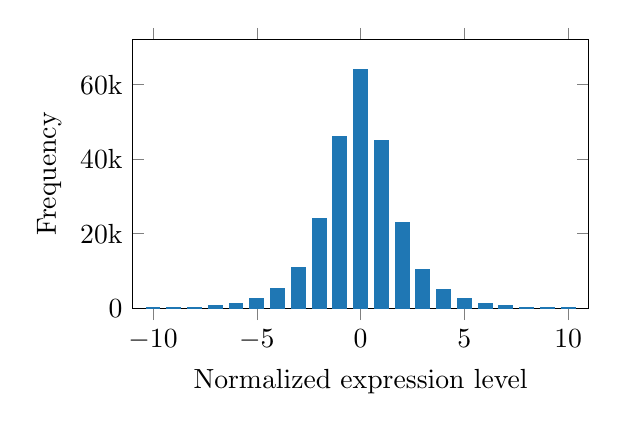
\begin{tikzpicture}
        \begin{axis}[
            ybar,
            width=5.80cm,
            height=3.41cm,
            scale only axis,
            bar width=4.98pt,
            ymin=0, ymax=72000,
            ytick={0, 20000, 40000, 60000},
            yticklabels={0, 20k, 40k, 60k},
            xmin=-11, xmax=11,
            xtick={-10, -5, 0, 5, 10},
            xlabel={Normalized expression level},
            ylabel={Frequency},
            scaled y ticks=false,
          ]
          \addplot[fill=geblue, draw=geblue, bar shift=0pt] coordinates {
              (-10, 80) (-9, 160) (-8, 320) (-7, 650) (-6, 1300) (-5, 2600)
              (-4, 5200) (-3, 11000) (-2, 24000) (-1, 46000) (0, 64000)
              (1, 45000) (2, 23000) (3, 10500) (4, 5000) (5, 2500)
              (6, 1250) (7, 620) (8, 300) (9, 150) (10, 70)
            };
        \end{axis}
      \end{tikzpicture}
    \end{column}

    \begin{column}{0.50\textwidth}
      Global distribution of the $39 \times 15{,}702$ expression values:
      \begin{itemize}
        \item Quasi-symmetric, centered ($\text{median} = 0.03$), bounded ($-10.43$ to $9.87$);
        \item Pre-normalized data (log-ratios) $\Rightarrow$ no non-linear transformation (log, Box-Cox) required; simple z-score standardization suffices.
      \end{itemize}
      \medskip
      \textit{Imputation} via training median (carried over to test): robust to outliers, strictly leak-free.
    \end{column}
  \end{columns}
\end{frame}

% Slide 10
\begin{frame}{Unsupervised PCA Fails to Separate Classes}
  \begin{columns}[c]
    \begin{column}{0.48\textwidth}
      \centering
      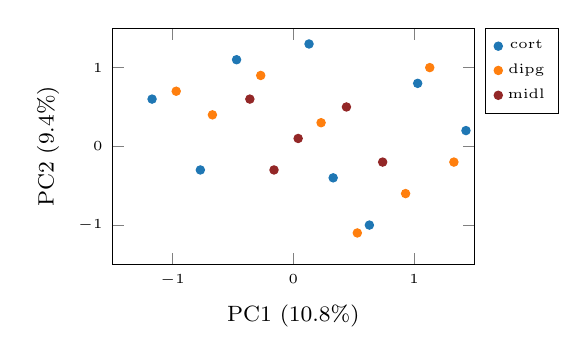
\begin{tikzpicture}
        \begin{axis}[
            scale only axis,
            width=4.6cm,
            height=3.0cm,
            xmin=-1.5, xmax=1.5,
            ymin=-1.5, ymax=1.5,
            xtick={-1, 0, 1},
            ytick={-1, 0, 1},
            xlabel={\footnotesize PC1 (10.8\%)},
            ylabel={\footnotesize PC2 (9.4\%)},
            legend pos=outer north east,
            legend style={font=\tiny},
            tick label style={font=\tiny}
          ]
          \addplot[only marks, mark=*, mark size=1.5pt, geblue] coordinates {
              (-1.17, 0.60) (-0.47, 1.10) (0.33, -0.40) (1.03, 0.80) (0.63, -1.00) (-0.77, -0.30) (1.43, 0.20) (0.13, 1.30)
            };
          \addplot[only marks, mark=*, mark size=1.5pt, dipgorange] coordinates {
              (0.23, 0.30) (0.93, -0.60) (-0.27, 0.90) (1.13, 1.00) (-0.67, 0.40) (0.53, -1.10) (1.33, -0.20) (-0.97, 0.70)
            };
          \addplot[only marks, mark=*, mark size=1.5pt, midlbrown] coordinates {
              (0.04, 0.10) (0.44, 0.50) (-0.16, -0.30) (0.74, -0.20) (-0.36, 0.60)
            };
          \legend{cort, dipg, midl}
        \end{axis}
      \end{tikzpicture}
    \end{column}

    \begin{column}{0.48\textwidth}
      \begin{itemize}
        \item PC1+PC2 capture only $\simeq 20\%$ of total variance for GE ($\simeq 27\%$ for CGH);
        \item The three point clouds \textbf{overlap heavily}; \texttt{midl} forms \textit{no distinct cluster}.
      \end{itemize}
      \medskip
      \begin{alertblock}{Consequence}
        \textit{Unsupervised} dimension reduction (PCA, Sparse PCA) projects variance along non-discriminative axes $\Rightarrow$ failure of Sparse PCA + LogReg pipelines. \textbf{A supervised projection is mandatory} (SGCCA).
      \end{alertblock}
    \end{column}
  \end{columns}
\end{frame}

% Slide 11
\begin{frame}{Real but Fragile Univariate Signal, High Redundancy}
  \begin{columns}[T]
    \begin{column}{0.50\textwidth}
      \boldmath{$t$}\textbf{-tests (Welch)} \texttt{\textbf{midl}} \textbf{vs. rest} (Welch due to unequal variances, $n_{\text{midl}} = 8$):
      \begin{itemize}
        \item \textbf{GE}: a few genes reach $|t| \simeq 4$–$5$ (e.g., \texttt{A\_32\_P85999}) $\Rightarrow$ univariate signal exists;
        \item \textbf{CGH}: statistics plateau around $|t| \simeq 3$, substantially weaker signal.
      \end{itemize}
      \bigskip
      \textbf{Strong intra-block redundancy} (correlated feature clusters, especially in CGH):
      \begin{itemize}
        \item Justifies \textbf{Elastic-Net} penalization
      \end{itemize}
    \end{column}

    \begin{column}{0.48\textwidth}
      \begin{exampleblock}{Univariate $\neq$ Robust Multivariate}
        With $p \gg n$ and $n_{\text{midl}} = 8$, these t-statistics are themselves noisy (a single patient can alter rankings) and do \textbf{not} account for multiplicity ($\sim 17{,}000$ tests). This is an exploratory diagnostic, not valid feature selection $\Rightarrow$ selection is delegated to penalized methods \textit{intra-CV}.
      \end{exampleblock}
    \end{column}
  \end{columns}
\end{frame}

% Slide 12
\begin{frame}{Univariate Signal around \texttt{midl}: Top Features (Welch's $t$)}
  \begin{columns}[T]
    \begin{column}{0.56\textwidth}
      \centering
      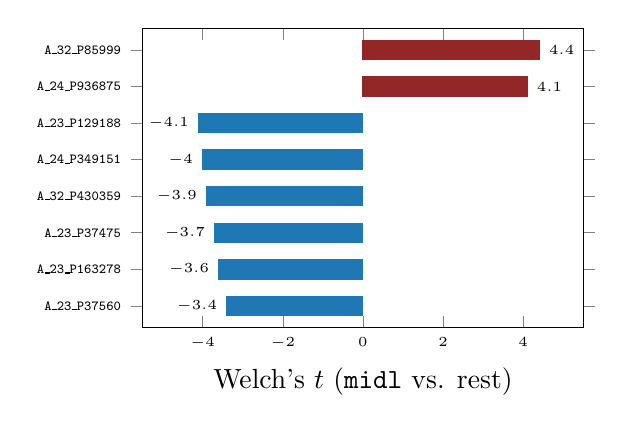
\begin{tikzpicture}
        \begin{axis}[
            xbar,
            bar shift=0pt,
            scale only axis,
            width=159.26pt,
            height=108.24pt,
            bar width=7pt,
            xmin=-5.5, xmax=5.5,
            xtick={-4, -2, 0, 2, 4},
            xlabel={Welch's $t$ (\texttt{midl} vs. rest)},
            ymin=0.4, ymax=8.6,
            ytick={1, 2, 3, 4, 5, 6, 7, 8},
            yticklabels={{A\_23\_P37560}, {A\_23\_P163278}, {A\_23\_P37475}, {A\_32\_P430359}, {A\_24\_P349151}, {A\_23\_P129188}, {A\_24\_P936875}, {A\_32\_P85999}},
            yticklabel style={font=\tiny\ttfamily},
            nodes near coords,
            nodes near coords style={/pgf/number format/fixed, font=\tiny},
            tick label style={font=\tiny}
          ]
          \addplot[draw=geblue, fill=geblue] coordinates {
              (-3.4, 1)
              (-3.6, 2)
              (-3.7, 3)
              (-3.9, 4)
              (-4, 5)
              (-4.1, 6)
            };
          \addplot[draw=midlbrown, fill=midlbrown] coordinates {
              (4.1, 7)
              (4.4, 8)
            };
        \end{axis}
      \end{tikzpicture}
    \end{column}

    \begin{column}{0.42\textwidth}
      \footnotesize
      \begin{itemize}
        \item \textbf{GE}: a few genes reach $|t| \simeq 4$–$5$; red = over-expressed in \texttt{midl} (e.g., \texttt{A\_32\_P85999}), with the majority under-expressed;
        \item \textbf{CGH}: statistics plateau around $|t| \simeq 3$, consistent with its near-total exclusion by sparse models.
      \end{itemize}
    \end{column}
  \end{columns}
\end{frame}

% Slide 13
\begin{frame}{Metric Selection: Balanced Accuracy}
  Raw \textit{accuracy} implicitly weights by class prevalence and would mask complete failure on \texttt{midl} (a trivial classifier never predicting midl already reaches $\simeq 11/14$).

  \medskip
  \begin{columns}[c]
    \begin{column}{0.54\textwidth}
      We adopt \textbf{macro-recall} (= balanced accuracy):
      \[
        \text{BA}(\hat{f}) = \frac{1}{|\mathcal{Y}|} \sum_{c \in \mathcal{Y}} \underbrace{\frac{|\{i : Y_i = c, \hat{f}(X_i) = c\}|}{|\{i : Y_i = c\}|}}_{\text{recall}_c}
      \]
      Equal weight assigned to all three classes, irrespective of prevalence.
    \end{column}

    \begin{column}{0.44\textwidth}
      \begin{alertblock}{An Example}
        For a classifier that \textit{never} predicts \texttt{midl}:
        \[
          \text{macro-recall} = \frac{1}{3}\left(\frac{5}{5} + \frac{6}{6} + \frac{0}{3}\right) = 0.667
        \]
      \end{alertblock}
    \end{column}
  \end{columns}
\end{frame}

% Slide 14: Section 3
\section{Formalism and Methodology}

% Slide 15
\begin{frame}{Probabilistic Framework and Bayes Classifier}
  \vspace{7pt}
  3-class classification: $(X_i, Y_i) \text{ i.i.d.} \sim P$, $X \in \mathbb{R}^p$, $Y \in \{1, 2, 3\}$. Risk of a classifier $f$ under loss $\ell$:
  \[
    R(f) = \mathbb{E}_{(X,Y)\sim P}[\ell(f(X), Y)], \qquad f^\star = \arg\min_f R(f).
  \]

  \bigskip
  \begin{block}{Under 0--1 Loss}
    With $\eta_c(x) = \mathbb{P}[Y = c \mid X = x]$, the Bayes optimal predictor is
    \[
      f^\star(x) = \arg\max_{c \in \mathcal{Y}} \eta_c(x).
    \]
    Since 0--1 loss is neither continuous nor differentiable, we optimize a convex, smooth \textbf{surrogate loss}: cross-entropy.
  \end{block}

  \bigskip
  \textit{Remark:} Under an \textit{asymmetric} loss (penalizing errors on \texttt{midl} more heavily), the Bayes predictor is no longer the argmax of $\eta_c$: this motivates cost-sensitive class weighting.
\end{frame}

% Slide 16
\begin{frame}{Multinomial Logistic Regression}
  Softmax model (with identifiability constraint $\beta_3 = 0$):
  \[
    \eta_c^\beta(x) = \mathbb{P}_\beta[Y = c \mid X = x] = \frac{e^{\beta_c^\top x}}{\sum_{k=1}^3 e^{\beta_k^\top x}}.
  \]
  Maximizing log-likelihood $\equiv$ minimizing empirical \textbf{cross-entropy}:
  \[
    \hat{R}_n(\beta) = -\frac{1}{n} \sum_{i=1}^n \log \eta_{Y_i}^\beta(X_i), \qquad \nabla_{\beta_c} \hat{R}_n(\beta) = \frac{1}{n} \sum_{i=1}^n \left( \eta_c^\beta(X_i) - \mathbf{1}_{\{Y_i = c\}} \right) X_i.
  \]
  \begin{itemize}
    \item \textbf{Convex and differentiable} objective; no closed-form solution $\Rightarrow$ Newton-Raphson method.
    \item \textbf{Linear} decision boundaries: $\hat{y} = \arg\max_c \hat{\beta}_c^\top x$.
  \end{itemize}
\end{frame}

% Slide 17
\begin{frame}{Weighted Likelihood: Inverse Prevalence Weights}
  The uniform empirical risk $\hat{R}_n$ is dominated by majority classes. We align the objective with balanced accuracy via
  \[
    \hat{R}_n^w(\beta) = -\frac{1}{n}\sum_{i=1}^n w_{Y_i} \log \eta_{Y_i}^\beta(X_i).
  \]

  \vspace{5pt}
  \begin{block}{Weights}
    Equalizing class contributions ($w_c n_c = \text{const}$) subject to normalization ($\sum_c w_c n_c = n$) yields
    \[
      w_c = \frac{n}{K\,n_c}, \qquad w_{\texttt{cort}} = 0.87, \quad w_{\texttt{dipg}} = 0.81, \quad w_{\texttt{midl}} = 1.62.
    \]
  \end{block}

  \bigskip
  The weighted gradient scales \texttt{midl} residuals by $w_{\texttt{midl}}$. This is theoretically more sound than synthetic oversampling like \texttt{SMOTE} (evaluated, inconclusive: synthesizing pseudo-patients in dimension 16,931 induces severe instability). Convexity is strictly preserved.
\end{frame}

% Slide 18
\begin{frame}{Elastic-Net Regularization and GLM Framework}
  \begin{columns}[T]
    \begin{column}{0.50\textwidth}
      \textbf{Elastic-Net} to control complexity in the $p \gg n$ regime:
      \[
        \min_\beta \left\{ \hat{R}_n(\beta) + \lambda\rho\|\beta\|_1 + \frac{\lambda(1-\rho)}{2}\|\beta\|_2^2 \right\}
      \]
      \vspace{0.2cm}
      \begin{itemize}
        \item $\ell_1$ (Lasso) $\Rightarrow$ feature \textbf{selection}
        \item $\ell_2$ (Ridge) $\Rightarrow$ \textbf{stability} under collinear features
        \item Non-differentiable $\ell_1$ $\Rightarrow$ proximal optimization (soft-thresholding).
      \end{itemize}
    \end{column}

    \begin{column}{0.48\textwidth}
      \begin{block}{GLM}
        Logistic regression is the canonical \textit{GLM}: $Y \mid X \sim \text{Categorical}$, logit link, $g(\mu_i) = x_i^\top \beta$. Log-likelihood is concave $\Rightarrow$ unique MLE obtained via Newton (iteratively reweighted least squares, IRLS).
      \end{block}
    \end{column}
  \end{columns}
\end{frame}

% Slide 19
\begin{frame}{Linear Discriminant Analysis (LDA)}
  Assumptions: conditional normality $X \mid Y = c \sim \mathcal{N}_p(\mu_c, \Sigma)$ and \textbf{homoscedasticity} ($\Sigma_c = \Sigma$). The discriminant function linearizes:
  \[
    \delta_c(x) = \underbrace{(\Sigma^{-1}\mu_c)^\top}_{w_c^\top} x - \underbrace{\left(\tfrac{1}{2}\mu_c^\top \Sigma^{-1}\mu_c - \log \pi_c\right)}_{b_c}, \qquad f^\star(x) = \arg\max_c w_c^\top x - b_c.
  \]
  Estimators: class priors $\hat{\pi}_c = \frac{n_c}{n}$, class centroids $\hat{\mu}_c$, and pooled covariance
  \[
    \hat{\Sigma} = \frac{1}{n-K} \sum_c \sum_i (X_i - \hat{\mu}_c)(X_i - \hat{\mu}_c)^\top \mathbf{1}_{Y_i = c}.
  \]

  \medskip
  \begin{alertblock}{Problem in $p \gg n$}
    $\hat{\Sigma}$ ($16{,}931 \times 16{,}931$) is \textbf{singular (non-invertible)}. LDA is therefore never applied directly to raw features, but rather to the low-dimensional \textit{supervised latent components} obtained via SGCCA.
  \end{alertblock}
\end{frame}

% Slide 20
\begin{frame}{Cross-Validation: Stratified, Repeated, Nested}
  With $n = 39$, any single train/validation split exhibits extreme variance.

  \bigskip
  \begin{columns}[T]
    \begin{column}{0.46\textwidth}
      \begin{itemize}
        \item \textbf{Stratification}: every fold preserves exact class proportions (preventing folds with zero \texttt{midl});
        \item \textbf{Repetition}: $K \times R = 7 \times 3 = 21$ folds to reduce the variance of $\hat{R}_{\text{CV}}$;
        \item \textbf{Metric}: balanced accuracy optimized and reported throughout.
      \end{itemize}
    \end{column}

    \begin{column}{0.50\textwidth}
      \begin{block}{Nested CV}
        \begin{itemize}
          \item \textit{Outer loop}: estimates $\hat{R}_{\text{CV}}$;
          \item \textit{Inner loop}: selects $\hat{\lambda} = \arg\min_\lambda \hat{R}_{\text{in}}(\lambda)$ strictly on the fold training split.
        \end{itemize}
        $\Rightarrow \hat{\lambda}$ is tuned without ever seeing test folds: zero \textbf{data leakage}. All feature selection is performed \textit{strictly within} cross-validation folds.
      \end{block}
    \end{column}
  \end{columns}
\end{frame}

% Slide 21
\begin{frame}{Multi-Block Fusion: From Naive Baselines to Cooperative Learning}
  Two blocks: $X \in \mathbb{R}^{n \times p_{\text{GE}}}$ and $Z \in \mathbb{R}^{n \times p_{\text{CGH}}}$.
  \begin{itemize}
    \item \textbf{Early fusion}: concatenate $[X \mid Z] \Rightarrow$ GE completely dominates; CGH is marginalized;
    \item \textbf{Late fusion}: separate model per block, then $\omega f_X + (1-\omega) f_Z \Rightarrow$ discards inter-block feature interactions.
  \end{itemize}

  \begin{block}{Cooperative Learning (Ding \& Tibshirani, PNAS 2022)}
    Continuous interpolation between early and late fusion via an \textbf{agreement penalty} $\rho \ge 0$ on predicted logits:
    \[
      J(\theta_x, \theta_z) = \hat{R}_{\text{CE}}(\theta_x, \theta_z) + \underbrace{\frac{\rho}{2} \|X \theta_x - Z \theta_z\|_F^2}_{\text{agreement}} + P_{\text{Elastic-Net}}(\theta_x, \theta_z).
    \]
    $\rho = 0$: early fusion; $\rho \to \infty$: late fusion. Equivalent to Elastic-Net optimization on \textit{augmented} feature data $(\tilde{X}, \tilde{z})$.
  \end{block}
\end{frame}

% Slide 22
\begin{frame}{SGCCA: The Supervised Latent Projection Framework}
  \textbf{Sparse Generalized CCA} (Tenenhaus \textit{et al.}): sparse components $y_j = X_j a_j$ maximizing inter-block covariance \textit{across connected blocks}:
  \[
    \max_{a_1, \dots, a_J} \sum_{j,k} c_{jk} g\left(\text{cov}(X_j a_j, X_k a_k)\right) \quad \text{s.t.} \quad \|a_j\|_2 \le 1, \; \|a_j\|_1 \le s_j.
  \]

  \begin{columns}[c]
    \begin{column}{0.54\textwidth}
      \begin{itemize}
        \item \textbf{3 blocks}: GE, CGH, and dummy label matrix $Y$ as a \textbf{supervised pivot};
        \item Design matrix: each molecular block is linked directly to $Y$, rather than linking GE--CGH directly
              \[
                C = \begin{pmatrix} 0 & 0 & 1 \\ 0 & 0 & 1 \\ 1 & 1 & 0 \end{pmatrix};
              \]
        \item $\ell_1$ budget $\Rightarrow$ variable selection; $\ell_2$ unit sphere $\Rightarrow$ stability;
        \item Block scaling $\tilde{X}_j = X_j / \sqrt{p_j}$ to balance block inertia.
      \end{itemize}
    \end{column}

    \begin{column}{0.44\textwidth}
      \centering
      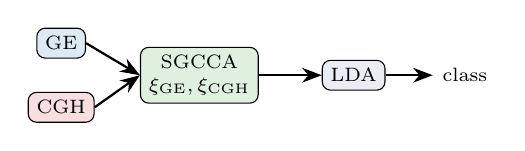
\begin{tikzpicture}[
        box/.style={rectangle, rounded corners=3pt, draw=black, align=center, font=\scriptsize, inner sep=3pt},
        arr/.style={-{Stealth[length=2.5mm]}, thick}
        ]
        \node[box, fill=boxblue] (ge) {GE};
        \node[box, fill=boxred, below=12pt of ge] (cgh) {CGH};
        \path (ge) -- (cgh) coordinate[midway] (mid);
        \node[box, fill=boxgreen, right=1.0cm of mid] (sgcca) {SGCCA \\ $\xi_{\text{GE}}, \xi_{\text{CGH}}$};
        \node[box, fill=boxlavender, right=0.8cm of sgcca] (lda) {LDA};
        \node[right=0.6cm of lda, font=\scriptsize] (classe) {class};

        \draw[arr] (ge.east) -- (sgcca.west);
        \draw[arr] (cgh.east) -- (sgcca.west);
        \draw[arr] (sgcca.east) -- (lda.west);
        \draw[arr] (lda.east) -- (classe.west);
      \end{tikzpicture}
      \vskip 4pt
        {\footnotesize Latent components feed into LDA in low-dimensional space, naturally bypassing the singularity of $\hat{\Sigma}$.}
    \end{column}
  \end{columns}
\end{frame}

% Slide 23: Section 4
\section{Results}

% Slide 24
\begin{frame}{Feature Selection and Pipeline Benchmark}
  Four supervised sparse pipelines evaluated under an identical protocol ($7 \times 3 = 21$ stratified folds, balanced accuracy, held-out test set $n = 14$). SGCCA selects \textbf{68 GE + 11 CGH} ($s_1 = 0.051$, $s_2 = 0.067$).

  \medskip
  \begin{center}
    \small
    \begin{tabular}{lcccc}
      \toprule
      \textbf{Method}                      & \textbf{CV bal\_acc} & \textbf{Test bal\_acc} & \texttt{\textbf{midl}} \textbf{test} & \textbf{N vars} \\
      \midrule
      Multinomial Lasso \textit{grouped}   & 0.784 $\pm$ 0.096    & 0.773                  & 0/3                                  & 27 GE           \\
      Multinomial Lasso \textit{ungrouped} & 0.838 $\pm$ 0.123    & 0.773                  & 0/3                                  & 27 GE           \\
      \rowcolor{boxgreen}
      Cooperative Lasso OvR ($\rho = 0$)   & 0.833 $\pm$ 0.129    & 0.924                  & 2/3                                  & 42 GE           \\
      \rowcolor{boxgreen}
      SGCCA + LDA                          & 0.829 $\pm$ 0.133    & 0.924                  & 2/3                                  & 68 GE + 11 CGH  \\
      \bottomrule
    \end{tabular}
  \end{center}

  \bigskip
  \begin{itemize}
    \item Only \textit{One-vs-Rest} or \textit{supervised latent space} pipelines recover the \texttt{midl} class (2/3);
    \item Switching the $\ell_1$ penalty from \textit{grouped} $\to$ \textit{ungrouped} gains +0.054 in CV (at the sole cost of a command-line flag), but yields identical test performance.
  \end{itemize}
\end{frame}

% Slide 25
\begin{frame}{Benchmark Performance}
  \begin{columns}[c]
    \begin{column}{0.48\textwidth}
      \centering
      {\footnotesize Balanced accuracy in CV ($\pm$ std dev)}
      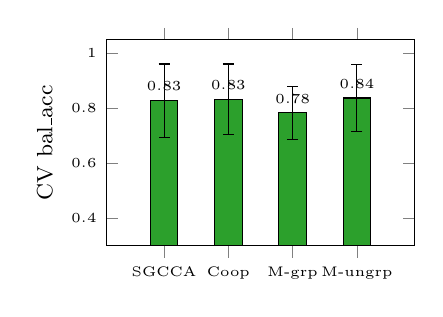
\begin{tikzpicture}
        \begin{axis}[
            ybar,
            width=5.5cm,
            height=4.2cm,
            bar width=10pt,
            ymin=0.3, ymax=1.05,
            ytick={0.4, 0.6, 0.8, 1},
            ylabel={\footnotesize CV bal\_acc},
            symbolic x coords={SGCCA,Coop,M-grp,M-ungrp},
            xtick=data,
            nodes near coords,
            nodes near coords style={/pgf/number format/fixed, /pgf/number format/precision=2, font=\tiny},
            enlarge x limits=0.3,
            tick label style={font=\tiny}
          ]
          \addplot[
            fill=midlgreen,
            draw=black,
            error bars/.cd,
            y dir=both,
            y explicit
          ] coordinates {
              (SGCCA, 0.829) +- (0, 0.133)
              (Coop, 0.833) +- (0, 0.129)
              (M-grp, 0.784) +- (0, 0.096)
              (M-ungrp, 0.838) +- (0, 0.123)
            };
        \end{axis}
      \end{tikzpicture}
    \end{column}

    \begin{column}{0.48\textwidth}
      \centering
      {\footnotesize Balanced accuracy on test set ($n = 14$)}
      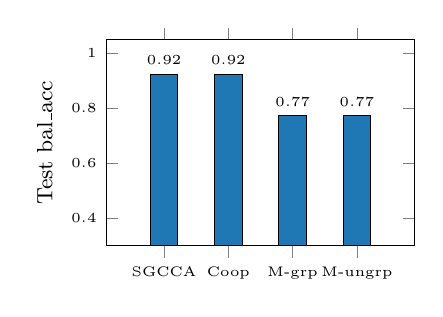
\begin{tikzpicture}
        \begin{axis}[
            ybar,
            width=5.5cm,
            height=4.2cm,
            bar width=10pt,
            ymin=0.3, ymax=1.05,
            ytick={0.4, 0.6, 0.8, 1},
            ylabel={\footnotesize Test bal\_acc},
            symbolic x coords={SGCCA,Coop,M-grp,M-ungrp},
            xtick=data,
            nodes near coords,
            nodes near coords style={/pgf/number format/fixed, /pgf/number format/precision=2, font=\tiny},
            enlarge x limits=0.3,
            tick label style={font=\tiny}
          ]
          \addplot[fill=geblue, draw=black] coordinates {
              (SGCCA, 0.924)
              (Coop, 0.924)
              (M-grp, 0.773)
              (M-ungrp, 0.773)
            };
        \end{axis}
      \end{tikzpicture}
    \end{column}
  \end{columns}

  \vfill
  \begin{center}
    \footnotesize In CV, three methods plateau around $\simeq 0.83$; on the test set, only \textbf{SGCCA + LDA} and \textbf{Cooperative OvR} achieve 0.924.
  \end{center}
\end{frame}

% Slide 26
\begin{frame}{Effective Sparsity: Retained Variables per Block}
  \begin{columns}[T]
    \begin{column}{0.54\textwidth}
      \centering
      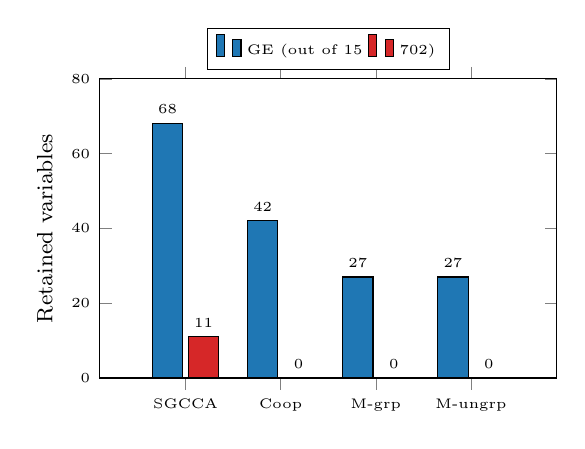
\begin{tikzpicture}
        \begin{axis}[
            ybar=2pt,
            width=5.8cm,
            height=3.8cm,
            scale only axis,
            bar width=11pt,
            ymin=0, ymax=80,
            ytick={0, 20, 40, 60, 80},
            ylabel={\footnotesize Retained variables},
            symbolic x coords={SGCCA,Coop,M-grp,M-ungrp},
            xtick=data,
            nodes near coords,
            nodes near coords style={/pgf/number format/fixed, font=\tiny},
            legend style={at={(0.5, 1.03)}, anchor=south, legend columns=2, font=\tiny},
            enlarge x limits=0.3,
            tick label style={font=\tiny}
          ]
          \addplot[fill=geblue] coordinates {(SGCCA, 68) (Coop, 42) (M-grp, 27) (M-ungrp, 27)};
          \addplot[fill=cghred] coordinates {(SGCCA, 11) (Coop, 0) (M-grp, 0) (M-ungrp, 0)};
          \legend{GE (out of 15,702), CGH (out of 1,229)}
        \end{axis}
      \end{tikzpicture}
    \end{column}

    \begin{column}{0.44\textwidth}
      All purely \textit{data-driven} methods spontaneously zero out the entire CGH block.

      \medskip
      Only \textbf{SGCCA} retains 11 CGH features: strictly because sparsity constraints $s_{\text{CGH}}$ are enforced block-by-block by design.

      \medskip
      Highly sparse and interpretable models ($\le 68$ features out of $\sim 17{,}000$).
    \end{column}
  \end{columns}
\end{frame}

% Slide 27
\begin{frame}{Cooperative Learning: An Instructive Instability}
  Under \texttt{multiview} (built on \texttt{glmnet}), the algorithm \textbf{diverges for any} $\rho > 0$ under the OvR formulation (\texttt{algorithm did not converge}). Two structural root causes:
  \begin{itemize}
    \item Newton weights $w_i = \hat{p}_i(1 - \hat{p}_i) \to 0$ on the rare class $\Rightarrow X^\top W X$ becomes nearly singular;
    \item The agreement penalty injects $\rho X^\top X$, amplifying already severe collinearity by a factor of $(1 + \rho)$.
  \end{itemize}

  \bigskip
  \begin{block}{Structural Insight}
    The $\ell_1$ penalty promotes \textit{sparsity} while the agreement penalty enforces \textit{view coupling}: antagonistic forces when GE and CGH share minimal common discriminant signal. Only $\rho = 0$ is viable (collapsing into standard OvR Lasso). The \textit{multinomial} formulation converges ($\rho^\star = 0.10$), but at lower balanced accuracy.
  \end{block}
\end{frame}

% Slide 28
\begin{frame}{Hyperparameter Sensitivity}
  \begin{columns}[T]
    \begin{column}{0.48\textwidth}
      \centering
      {\footnotesize Multinomial Lasso: $\alpha$ sweep}
      \vskip 4pt
      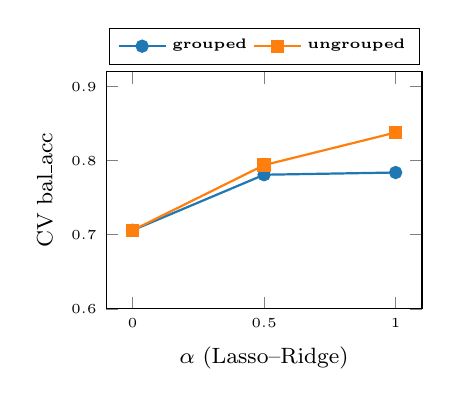
\begin{tikzpicture}
        \begin{axis}[
            width=4.01cm,
            height=3.01cm,
            scale only axis,
            xmin=0, xmax=1,
            ymin=0.6, ymax=0.92,
            enlarge x limits=0.1,
            enlarge y limits=false,
            xtick={0, 0.5, 1},
            ytick={0.6, 0.7, 0.8, 0.9},
            xlabel={\footnotesize $\alpha$ (Lasso–Ridge)},
            ylabel={\footnotesize CV bal\_acc},
            legend style={at={(0.5, 1.03)}, anchor=south, legend columns=2, font=\tiny},
            tick label style={font=\tiny}
          ]
          \addplot[thick, geblue, mark=*, mark size=2pt] coordinates {(0, 0.706) (0.5, 0.781) (1.0, 0.784)};
          \addplot[thick, dipgorange, mark=square*, mark size=2pt] coordinates {(0, 0.706) (0.5, 0.794) (1.0, 0.838)};
          \legend{\textbf{grouped}, \textbf{ungrouped}}
        \end{axis}
      \end{tikzpicture}
      \vskip 2pt
        {\footnotesize At $\alpha = 1$, switching \textit{grouped} $\to$ \textit{ungrouped}: +0.054.}
    \end{column}

    \begin{column}{0.48\textwidth}
      \centering
      {\footnotesize Cooperative OvR: $\rho$ sweep}
      \vskip 4pt
      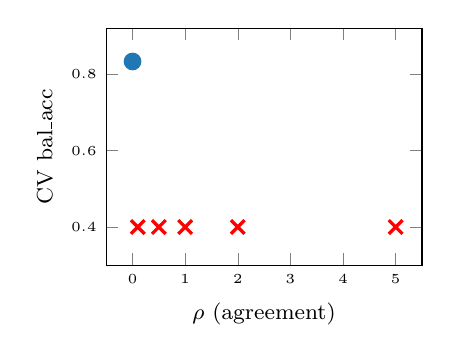
\begin{tikzpicture}
        \begin{axis}[
            width=4.01cm,
            height=3.01cm,
            scale only axis,
            xmin=0, xmax=5,
            ymin=0.3, ymax=0.92,
            enlarge x limits=0.1,
            enlarge y limits=false,
            xtick={0, 1, 2, 3, 4, 5},
            ytick={0.4, 0.6, 0.8},
            xlabel={\footnotesize $\rho$ (agreement)},
            ylabel={\footnotesize CV bal\_acc},
            tick label style={font=\tiny}
          ]
          \addplot[only marks, mark=*, mark size=3pt, geblue] coordinates {(0, 0.833)};
          \addplot[only marks, mark=x, mark size=3.5pt, red, line width=1.2pt] coordinates {
              (0.1, 0.4) (0.5, 0.4) (1, 0.4) (2, 0.4) (5, 0.4)
            };
        \end{axis}
      \end{tikzpicture}
      \vskip 2pt
        {\footnotesize Red crosses: solver non-convergence (\texttt{multiview}/\texttt{glmnet}); only $\rho = 0$ is viable.}
    \end{column}
  \end{columns}
\end{frame}

% Slide 29
\begin{frame}{Multinomial vs. OvR: The Rare Class Bottleneck}
  \vspace{15pt}
  Identical loss formulations yield divergent behaviors in $p \gg n$ under severe class imbalance.

  \medskip
  \begin{columns}[c]
    \begin{column}{0.48\textwidth}
      \centering
      \textbf{SGCCA + LDA / Cooperative OvR}
      \vskip 2pt
      \small
      \setlength{\tabcolsep}{7pt}
      \begin{tabular}{lccc}
                        & p.\texttt{cort}          & p.\texttt{dipg}          & p.\texttt{midl}                 \\
        t.\texttt{cort} & \cellcolor{lightgeblue}5 & 0                        & 0                               \\
        t.\texttt{dipg} & 0                        & \cellcolor{lightgeblue}6 & 0                               \\
        t.\texttt{midl} & 0                        & 1                        & \cellcolor{cellgreen}\textbf{2} \\
      \end{tabular}
      \vskip 2pt
      bal\_acc = 0.924: \texttt{midl} 2/3
    \end{column}

    \begin{column}{0.48\textwidth}
      \centering
      \textbf{Multinomial Lasso (grouped/ungrouped)}
      \vskip 2pt
      \small
      \setlength{\tabcolsep}{7pt}
      \begin{tabular}{lccc}
                        & p.\texttt{cort}          & p.\texttt{dipg}          & p.\texttt{midl}           \\
        t.\texttt{cort} & \cellcolor{lightgeblue}5 & 0                        & 0                         \\
        t.\texttt{dipg} & 0                        & \cellcolor{lightgeblue}6 & 0                         \\
        t.\texttt{midl} & 1                        & \cellcolor{cellred}2     & \cellcolor{celllightred}0 \\
      \end{tabular}
      \vskip 2pt
      bal\_acc = 0.773: \texttt{midl} 0/3
    \end{column}
  \end{columns}

  \medskip
  \begin{exampleblock}{The OvR "Safety Net"}
    In OvR, a \texttt{midl}-vs-rest sub-classifier with zero coefficients maintains an \textit{intercept} calibrated to training prevalence:
    $\hat{P}_{\texttt{midl}} \simeq \sigma(\log(8/31)) \simeq 0.205$ \textit{constant}.
    When \texttt{cort} and \texttt{dipg} reject an ambiguous patient, this baseline probability wins the $\arg\max$ decision (e.g., P11, P19). Conversely, the multinomial sum-to-one constraint $\sum_c P_c = 1$ pulls this unallocated probability mass toward \texttt{dipg}.
  \end{exampleblock}
\end{frame}

% Slide 30
\begin{frame}{Rescuing midl: Predicted Class Probabilities (Cooperative OvR)}
  \begin{columns}[T]
    \begin{column}{0.54\textwidth}
      \centering
      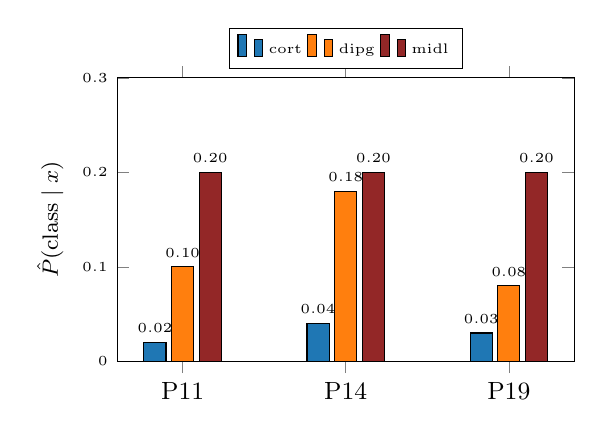
\begin{tikzpicture}
        \begin{axis}[
            ybar=2pt,
            width=5.8cm,
            height=3.6cm,
            scale only axis,
            bar width=8pt,
            ymin=0, ymax=0.3,
            ytick={0, 0.1, 0.2, 0.3},
            ylabel={\footnotesize $\hat{P}(\text{class} \mid x)$},
            symbolic x coords={P11,P14,P19},
            xtick=data,
            nodes near coords,
            nodes near coords style={/pgf/number format/fixed, /pgf/number format/precision=2, /pgf/number format/zerofill=true, font=\tiny},
            legend style={at={(0.5, 1.03)}, anchor=south, legend columns=3, font=\tiny},
            enlarge x limits=0.2,
            xticklabel style={font=\small},
            yticklabel style={font=\tiny}
          ]
          \addplot[fill=geblue] coordinates {(P11, 0.02) (P14, 0.04) (P19, 0.03)};
          \addplot[fill=dipgorange] coordinates {(P11, 0.10) (P14, 0.18) (P19, 0.08)};
          \addplot[fill=midlbrown] coordinates {(P11, 0.20) (P14, 0.20) (P19, 0.20)};
          \legend{cort, dipg, midl}
        \end{axis}
      \end{tikzpicture}
    \end{column}

    \begin{column}{0.44\textwidth}
      For the 3 true test \texttt{midl} patients, OvR yields an almost constant baseline probability
      \[
        \hat{P}_{\texttt{midl}} \simeq \sigma(\log(8/31)) \simeq 0.205.
      \]
      With \texttt{cort} and \texttt{dipg} rejected, this baseline wins via \textbf{argmax} (P11, P19).

      \bigskip
      Multinomial models, bound by $\sum_c P_c = 1$, drain this mass into \texttt{dipg} $\Rightarrow$ \texttt{midl} recall = 0/3.
    \end{column}
  \end{columns}
\end{frame}

% Slide 31: Section 5
\section{Stability and Reproducibility}

% Slide 32
\begin{frame}{Stability of Feature Selection}
  In the $p \gg n$ regime, selected feature sets exhibit variance under perturbations. We quantify stability via \textbf{bootstrap resampling} (Efron, 1979): selection frequency $\hat{\Pi}_k = \frac{1}{B} \sum_b \mathbf{1}_{\{a_k^{(b)} \ne 0\}}$, stable set $= \{k : \hat{\Pi}_k \ge \pi_{\text{thr}}\}$ (Meinshausen \& Bühlmann, 2010; $\pi_{\text{thr}} = 0.6$, $B = 200$).

  \bigskip
  \begin{columns}[T]
    \begin{column}{0.50\textwidth}
      \centering
      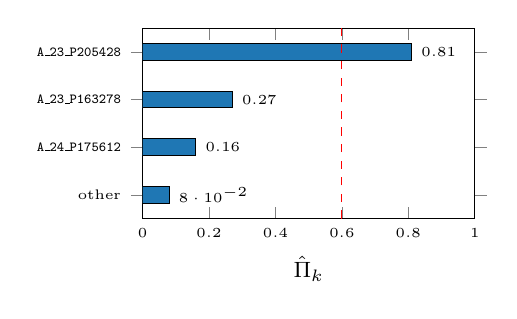
\begin{tikzpicture}
        \begin{axis}[
            xbar,
            width=5.8cm,
            height=4.0cm,
            bar width=6pt,
            xmin=0, xmax=1,
            xtick={0, 0.2, 0.4, 0.6, 0.8, 1},
            xlabel={\footnotesize $\hat{\Pi}_k$},
            ymin=0.5, ymax=4.5,
            ytick={1, 2, 3, 4},
            yticklabels={other, {\texttt{A\_24\_P175612}}, {\texttt{A\_23\_P163278}}, {\texttt{A\_23\_P205428}}},
            nodes near coords,
            nodes near coords style={font=\tiny},
            tick label style={font=\tiny}
          ]
          \addplot[fill=geblue] coordinates {
              (0.08, 1)
              (0.16, 2)
              (0.27, 3)
              (0.81, 4)
            };
          \draw[red, dashed] (axis cs:0.6, 0.5) -- (axis cs:0.6, 4.5);
        \end{axis}
      \end{tikzpicture}
      \vskip 2pt
        {\footnotesize OvR Lasso: one stable top gene (\texttt{A\_23\_P205428}, $\hat{\Pi} \simeq 0.81$).}
    \end{column}

    \begin{column}{0.48\textwidth}
      \begin{itemize}
        \item A \textbf{core set of GE genes} is consistently selected;
        \item \textbf{SGCCA}: \textit{more} stable core (3 genes $> \pi_{\text{thr}}$, sharing the same top gene as Lasso $\Rightarrow$ cross-method concordance);
        \item The \textbf{exclusion of CGH} by data-driven models is \textit{remarkably stable}: a genuine finding, not an artifact.
      \end{itemize}
    \end{column}
  \end{columns}
\end{frame}

% Slide 33
\begin{frame}{Is the Signal Genuine? Permutation Testing}
  \vspace{14pt}
  \begin{columns}[T]
    \begin{column}{0.53\textwidth}
      \textbf{Permutation test} (Ojala \& Garriga, 2010):
      \begin{itemize}
        \item $H_0$: no statistical association between features and labels (expected BA = 1/3);
        \item Permute labels, retrain the entire pipeline from scratch, $B = 500$ repetitions;
        \item \textbf{p-value} = fraction of permutations matching or exceeding observed score.
      \end{itemize}

      \medskip
      \begin{block}{Result}
        All models: \textbf{p-value} = 0.002. We reject $H_0$: predictive signal is statistically significant and \textit{not attributable to chance}, despite $p \gg n$.
      \end{block}
    \end{column}

    \begin{column}{0.43\textwidth}
      \begin{exampleblock}{Reproducibility}
        Fixed random seeds (CV splits, bootstrap, solver initializations) $\Rightarrow$ exactly reproducible numbers.
      \end{exampleblock}

      \begin{alertblock}{Robust vs. Fragile}
        \textbf{Robust}: primary signal driven by GE; CGH uninformative; clear \texttt{cort}/\texttt{dipg} separation; global significance.

        \medskip
        \textbf{Fragile}: fine ranking among top methods; exact \texttt{midl} recall (hinges on 1–2 test patients); exact gene list (stable core, volatile periphery).
      \end{alertblock}
    \end{column}
  \end{columns}
\end{frame}

% Slide 34: Section 6
\section{Literature Review}

% Slide 35
\begin{frame}{Literature Review: Foundations and Positioning}
  Every methodological design choice is grounded in established literature:
  \begin{description}
    \item[\textbf{Supervised multi-block integration}] RGCCA (Tenenhaus \& Tenenhaus, \textit{Psychometrika}, 2011); SGCCA / variable selection (Tenenhaus \textit{et al.}, \textit{Biostatistics}, 2014); block relaxation (De Leeuw, 1994; Tenenhaus \textit{et al.}, 2017; Girka \textit{et al.}, 2024; thresholding: Gloaguen \textit{et al.}, 2017).
    \item[\textbf{Cooperative learning}] Multi-view cooperative learning (Ding, Li, Narasimhan \& Tibshirani, \textit{PNAS}, 2022).
    \item[\textbf{Regularization \& GLM}] Lasso / Elastic-Net with proximal gradient descent; multinomial logistic regression (GLM, logit link); class weighting via \texttt{class\_weight="balanced"}.
    \item[\textbf{Stability \& validation}] Bootstrap (Efron, 1979); stability selection (Meinshausen \& Bühlmann, 2010); permutation testing (Ojala \& Garriga, 2010).
  \end{description}

  \begin{columns}[T]
    \begin{column}{0.48\textwidth}
      \textbf{Direct lineage}: identical dataset (IGR pediatric gliomas) and experimental setting as the RGCCA case study; SGCCA + LDA \textbf{reproduces} the published benchmark (CV $\simeq 0.826 \pm 0.136$, test $\simeq 91.7\%$).
    \end{column}
    \begin{column}{0.48\textwidth}
      \textbf{Contributions}: rigorous cross-family benchmark; algorithmic diagnosis of Cooperative divergence for $\rho > 0$; analytical breakdown of OvR vs. multinomial for rare class \texttt{midl}; stability analysis beyond point accuracy.
    \end{column}
  \end{columns}

  \smallskip
  \textit{Comprehensive bibliography provided in the full report.}
\end{frame}

% Slide 36
\begin{frame}{Conclusion}
  \begin{block}{Key Takeaways}
    \begin{itemize}
      \item \textbf{Challenging setting}: $p \gg n$ + multi-omics + rare class \texttt{midl};
      \item \textbf{SGCCA + LDA}: selected model: highest overall accuracy (test $\simeq 0.924$) \textit{and} highest stability, with \texttt{midl} recall of 2/3;
      \item \textbf{Sparse and interpretable} model ($\simeq 68$ genes, 11 CGH regions);
      \item Signal rigorously validated via permutation test ($p \simeq 0.002$).
    \end{itemize}
  \end{block}

  \medskip
  \textbf{Future Directions:}
  \begin{itemize}
    \item Validation on external patient cohorts; biological pathway analysis of stable core genes;
    \item Multi-component SGCCA; integration of a 3rd block (clinical covariates).
  \end{itemize}

  \vfill
  \begin{center}
    {\large \textbf{Thank you for your attention!}}
  \end{center}
\end{frame}

\end{document}
